% !TEX root=../thesis.tex

\chapter{Research Methods} % (fold)
% Research questions and method
\label{cha:research_questions_and_method}
This chapter describes the basic research method used in this 
thesis. We will then describe how the method was used.
\section{Research Methods} % (fold)
\label{sec:research_method}

During this research we applied the Design Science Research Process (DSRP) as the research method. 
This is based on 6 steps which are presented in the list
below. Depending on what the focus of the project is, the project can start at
almost any of the steps below.\cite{peffers2006design}

\begin{description}
	\item [1. Problem identification and motivation] Defines the problem to be
	researched. 
	\item [2. Objectives of a solution] Infer the goals of the solution.
	\item [3. Design and development] Creates a artifact for the solution.
	\item [4. Demonstration] Demonstrate the created artifact.
	\item [5. Evaluation] Observe and measure how the artifact gives a solution 
	to the problem.
	\item [6. Communication] Communicate the problem along with the artifact.
\end{description}

As Hevner, March, Park, and Ram\cite{von2004design} describes, 
evaluation of a product, produced through a sequence of expert activities 
provides feedback information and a better understanding of the problem in 
order to the quality of the product. This means that one have a process loop
which is typically iterated a number of times before the final design artifact
is generated. This is demonstrated in \Ref{fig:DSRP}, where one can see the
loop as going from Step 2 (Objectives of a solution) to Step 5 (Evaluation) and
back.

\begin{figure}[!htbp]
	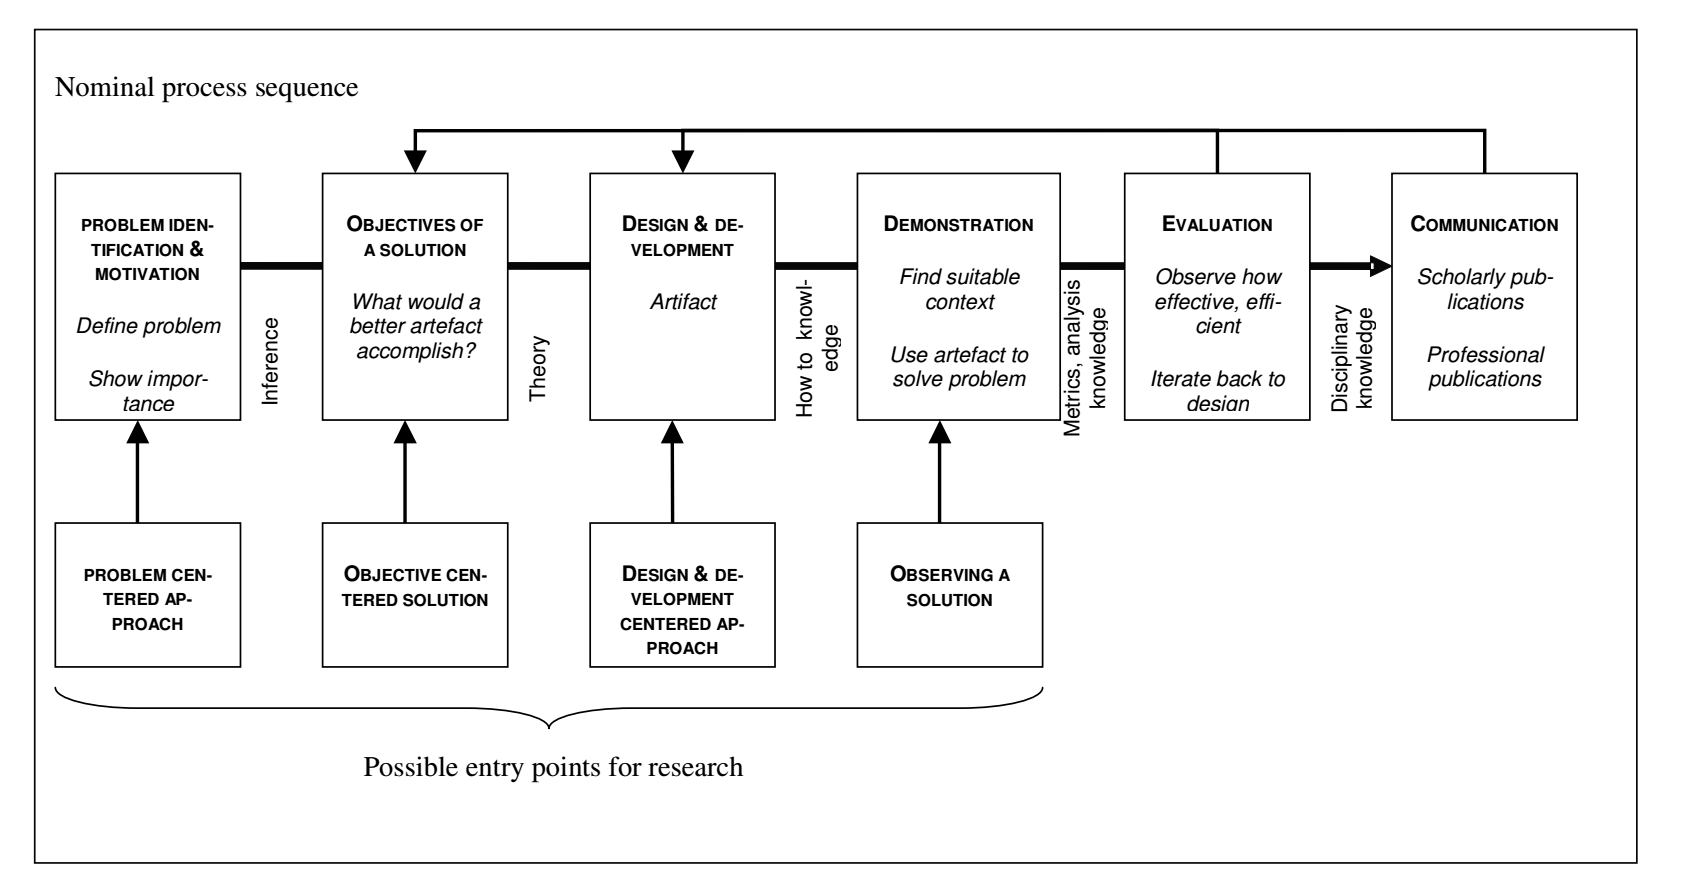
\includegraphics[width=\textwidth,center]{dsrp_modell.png}
	\caption[Design science research process (DSRP) model]{Design research process (DSRP)
	model\cite{peffers2006design}}
	\label{fig:DSRP}
\end{figure}


% section research_method (end)

\section{Project Research} % (fold)
\label{sec:workshops}
In this thesis, the problem was 
identified and motivated prior to the thesis, thus the natural starting 
point of this research was to go into the second stage called objective 
centered. \Ref{fig:DSRP} shows four entry points into a design 
research process; Problem centered-, objective centered-, design\&development-
centered-approach and observing a solution. 

This thesis was an interaction between objectives of a solution, and a study of prior 
art. Examining the state-of-the-art… XXX\\
At first a case study of similar 
systems was performed. These systems where then categorized into frameworks to 
cover the functionality and what information was presented. Based on these 
frameworks, the initial goals were defined.\\

%The second step performed of defining the goals of the solution and the
%prototype was to have two workshops. These workshops were meant to further 
%define the needs of the stakeholders and define the goals for the prototype.
%Participating on these workshops were several stakeholders which helped define
%the direction of the process.

Since the part of determining the needs and requirements of the stakeholders 
are a important deal of having a stakeholder aware system, it is important to
define these, such as by doing a requirements elicitation. To help define both 
which stakeholders were relevant for the system to beware of, and the needs of 
these stakeholders, a focus groups was put together and met for a discussion
during a workshop. As Goguen and Linde \cite{goguen1993techniques} says, such 
groups have a claim to greatly accelerate the development of requirements.

%Fix '... these defined..' !!!
By having these discussions, one is able to help define specifications for the
system and define the domain. As Zave and Jackson \cite{zave1997four} 
conclude, by having these defined and validated against the environment, we
are guaranteed that if the specification is implemented as an artifact which
is connected to the environment, the requirements will be satisfied. \\


As part of the iterative loop, a meeting with the supervisors were held each 
week where the continued development of a prototype was demonstrated and 
evaluated against the objectives of the solution. Based on the evaluation that 
took place during these meetings, the process was returned to step 2 or 3 
where the objectives and design were looked at again and optimally redefined.

% section workshops (end)

% chapter research_questions_and_method (end)

